% Created 2024-02-07 Wed 07:42
% Intended LaTeX compiler: pdflatex
\documentclass[presentation]{beamer}
\usepackage[utf8]{inputenc}
\usepackage[T1]{fontenc}
\usepackage{graphicx}
\usepackage{longtable}
\usepackage{wrapfig}
\usepackage{rotating}
\usepackage[normalem]{ulem}
\usepackage{amsmath}
\usepackage{amssymb}
\usepackage{capt-of}
\usepackage{hyperref}
\mode<beamer>{\usetheme{Madrid}}
\definecolor{SUred}{rgb}{0.59375, 0, 0.17969} % SU red (primary)
\definecolor{SUblue}{rgb}{0, 0.17578, 0.38281} % SU blue (secondary)
\setbeamercolor{palette primary}{bg=SUred,fg=white}
\setbeamercolor{palette secondary}{bg=SUblue,fg=white}
\setbeamercolor{palette tertiary}{bg=SUblue,fg=white}
\setbeamercolor{palette quaternary}{bg=SUblue,fg=white}
\setbeamercolor{structure}{fg=SUblue} % itemize, enumerate, etc
\setbeamercolor{section in toc}{fg=SUblue} % TOC sections
% Override palette coloring with secondary
\setbeamercolor{subsection in head/foot}{bg=SUblue,fg=white}
\setbeamercolor{date in head/foot}{bg=SUblue,fg=white}
\institute[SU]{Shenandoah University}
\titlegraphic{\includegraphics[width=0.5\textwidth]{\string~/Documents/suLogo/suLogo.pdf}}
\newcommand{\R}{\mathbb{R}}
\usepackage{tikz}
\usetheme{default}
\author{Chase Mathison\thanks{cmathiso@su.edu}}
\date{7 February 2024}
\title{The Other Trig Functions, Pt. 2}
\hypersetup{
 pdfauthor={Chase Mathison},
 pdftitle={The Other Trig Functions, Pt. 2},
 pdfkeywords={},
 pdfsubject={},
 pdfcreator={Emacs 29.1 (Org mode 9.6.7)}, 
 pdflang={English}}
\begin{document}

\maketitle

\section{Announcements}
\label{sec:org1729c50}
\begin{frame}[label={sec:org34ed8b9}]{Announcements}
\begin{enumerate}
\item Homework in M.O.M.
\item Quiz on Friday.
\end{enumerate}
\end{frame}

\section{Lecture}
\label{sec:org6357d3b}
\begin{frame}[label={sec:org734230a}]{Alternate Pythagorean Identity}
\end{frame}

\begin{frame}[label={sec:org050a0bd}]{Alternate Pythagorean Identities}
\begin{block}{Alternate Pythorean Identities}
\[ 1 + \left( \tan\theta \right)^2 = \left( \sec\theta \right)^2 \]
\[ \left( \cot\theta \right)^2 + 1 = \left( \csc\theta \right)^2 \]
\end{block}
\end{frame}

\begin{frame}[label={sec:org4b8d907}]{Example}
\end{frame}

\begin{frame}[label={sec:org1014581}]{Period of the Trig Functions}
\begin{columns}
\begin{column}{0.45\columnwidth}
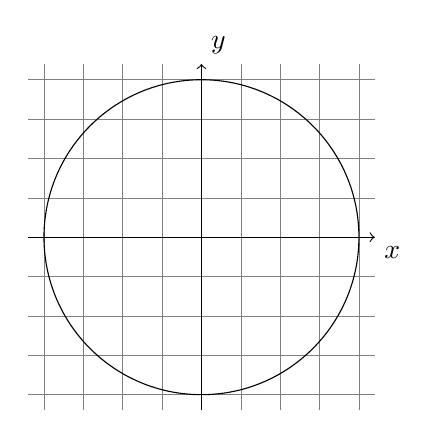
\begin{tikzpicture}[scale=2]
  \draw[help lines,step=0.25] (-1.1,-1.1) grid (1.1,1.1);
  \draw[->] (-1.1,0) -- (1.1,0) node [anchor=north west] {$x$};
  \draw[->] (0,-1.1) -- (0,1.1) node [anchor=south west] {$y$};
  \draw (0,0) circle [radius=1];
\end{tikzpicture}
\end{column}
\begin{column}{0.45\columnwidth}
\begin{block}{Period of Trig Functions}
The \uline{\hspace*{1in}} of a ``repeating'' function \(f(x)\) is the smallest
positive number \(P\) such that
\[
f(x + P) = \hspace{1in}\]

The period of \(\sin(\theta), \cos(\theta), \sec(\theta)\) and
\(\csc(\theta)\) is \uline{\hspace*{1in}}.

The period of \(\tan(\theta)\) and \(\cot(\theta)\) is \uline{\hspace*{1in}}.
\end{block}
\end{column}
\end{columns}
\end{frame}

\begin{frame}[label={sec:org09a6200}]{Example}
\end{frame}

\begin{frame}[label={sec:org162ec93}]{Example}
Simplify the following expressions using fundamental trig identities:
\begin{enumerate}
\item \(\tan(\theta)\cos(\theta)\)
\item \(\frac{\csc(\theta)}{\sec(\theta)}\)
\item \(\sin(\theta)\csc(\theta) + \frac{1}{(\cos(\theta))^2}\)
\end{enumerate}
\vspace{10in}   
\end{frame}

\begin{frame}[label={sec:orgc9d527f}]{Example}
Suppose \(\tan(\alpha) = \frac{-3}{5}\) and \(\frac{\pi}{2} \le \alpha \le \pi\).  Find
the other 5 trig functions at \(\alpha\).  (Hint: Find \(\sec(\alpha)\) first.)
\vspace{10in}
\end{frame}

\begin{frame}[label={sec:org9c068fe}]{Example}
\end{frame}

\begin{frame}[label={sec:orgec370d5}]{Right Triangle Trigonometry}
Let's look one more time at the unit circle:

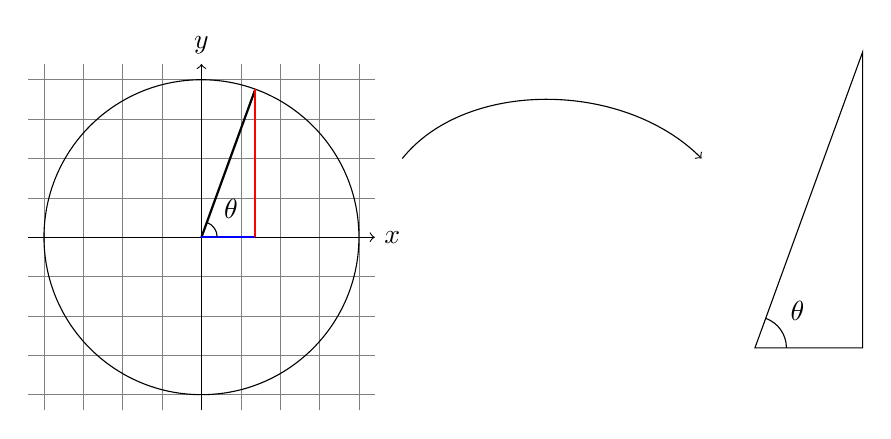
\begin{tikzpicture}[scale=2]
  \draw[help lines,step=0.25] (-1.1,-1.1) grid (1.1,1.1);
  \draw[->] (-1.1,0) -- (1.1,0) node [anchor=west] {$x$};
  \draw[->] (0,-1.1) -- (0,1.1) node [anchor=south] {$y$};
  \draw (0,0) circle [radius=1];
  \draw[thick] (0,0) -- (70:1);
  \draw[color=blue,thick] (0,0) -- (70:1 |- 0,0);
  \draw[color=red,thick] (70:1) -- (70:1 |- 0,0);
  \draw[xshift=5,->] (1.1,0.5) .. controls (1.5,1) and (2.5,1)  .. (3,0.5);
  \draw (0.1,0) arc [start angle = 0,end angle = 70,radius=0.1];
  \node [anchor = south west] at (35:0.1) {$\theta$};
  \begin{scope}[scale=2,xshift=50,yshift=-10]
    \draw (0,0) -- (70:1) -- (70:1 |- 0,0) -- cycle;
    \draw (0.1,0) arc [start angle = 0,end angle = 70,radius=0.1];
    \node [anchor = south west] at (35:0.1) {$\theta$};
  \end{scope}
\end{tikzpicture}
\end{frame}

\begin{frame}[label={sec:org30f16ff}]{SOHCAHTOA}
A convenient way to remember Sine/Cosine/Tangent with right triangles is the
memory device \uline{\hspace*{1in}}.

\vspace{0.5in}
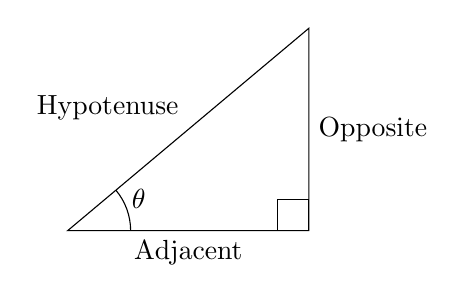
\begin{tikzpicture}[scale=4]
  \draw (0,0) -- node [anchor=south east] {Hypotenuse} (40:1) -- node [anchor = west] {Opposite} (40:1 |- 0,0) --  node [anchor=north] {Adjacent} cycle;
  \draw (0.2,0) arc [start angle = 0,end angle = 40,radius=0.2];
  \node [anchor = west] at (30:0.2) {$\theta$};
  \draw (40:1 |- 0,0) rectangle ++(-0.1,0.1);
\end{tikzpicture}
\end{frame}


\begin{frame}[label={sec:orgb21c62e}]{Example}
Find \(\sin(\alpha), \cos(\alpha)\) and \(\tan(\alpha)\) from the following triangle:
\vspace{0.5in}

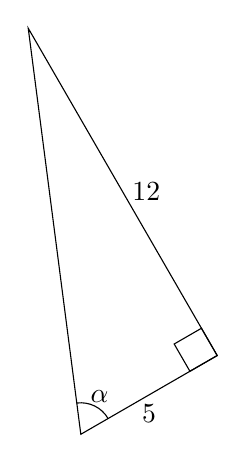
\begin{tikzpicture}[scale=0.4,rotate=30]
  \draw (0,0) -- node[anchor=north] {$5$} (5,0) -- node[anchor=west] {$12$} (5,12) -- cycle;
  \draw (1,0) arc [start angle = 0,end angle = 67.38, radius = 1];
  \draw (5,0) rectangle ++(-1,1);
  \node [anchor=west] at (60:1.2) {$\alpha$};
\end{tikzpicture}
\end{frame}

\begin{frame}[label={sec:org5423d6b}]{The other trig functions}
We can also find \(\sec(\theta), \csc(\theta)\) and \(\cot(\theta)\) using right triangles
and the fact that
\[
\sec(\theta) = \hspace{1in}\]
\[
\csc(\theta) = \hspace{1in} \]
\[
\cot(\theta) = \hspace{1in} \]
\end{frame}

\begin{frame}[label={sec:orge80e543}]{Example}
For \(\theta\) given below, find all 6 trig functions:

\vspace{0.5in}
\begin{tikzpicture}[scale=0.2]
  \draw (0,0) -- node[anchor = north] {20} (20,0) -- node[anchor=west] {21} (20,21) -- cycle;
  \draw (20,0) rectangle ++(-2,2);
  \draw (0,0) ++(5,0) arc[start angle=0,end angle = 46.4,radius=5];
  \path (0,0) ++(30:5) node [anchor = west] {$\theta$};
\end{tikzpicture}
\end{frame}

\begin{frame}[label={sec:orgbf931f8}]{Example}
Let's look at a few special triangles:

\begin{tikzpicture}[scale=4]
  \draw (0,0) -- (45:1) -- (45:1 |- 0,0) -- cycle;
  \draw[xshift=40] (0,0) -- (60:1) -- (60:1 |- 0,0) -- cycle;
\end{tikzpicture}
\end{frame}

\begin{frame}[label={sec:orgac17a4f}]{Example}
Find the missing side lengths in the following right triangle:

\vspace{0.5in}
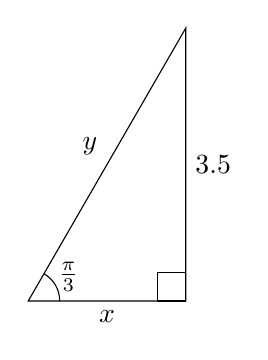
\begin{tikzpicture}[scale=4]
  \draw (0,0) -- node [anchor=south east] {$y$} (60:1) -- node[anchor = west] {3.5} (60:1 |- 0,0) -- node [anchor=north] {$x$} cycle;
  \draw (0.1,0) arc (0:60:0.1);
  \draw (60:1 |- 0,0) rectangle ++(-0.09,0.09);
  \node[anchor = west] at (50:0.1) {$\frac{\pi}{3}$};
\end{tikzpicture}
\end{frame}

\begin{frame}[label={sec:org8fca351}]{A Special Relationship}
Let's look at something very special that we can see now between Sine and Cosine

\vspace{0.5in}
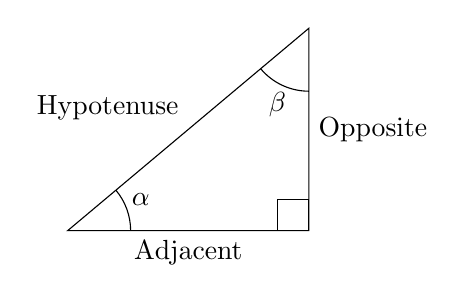
\begin{tikzpicture}[scale=4]
  \draw (0,0) -- node [anchor=south east] {Hypotenuse} (40:1) -- node [anchor = west] {Opposite} (40:1 |- 0,0) --  node [anchor=north] {Adjacent} cycle;
  \draw (0.2,0) arc [start angle = 0,end angle = 40,radius=0.2];
  \draw (40:1) ++(-90:0.2) arc [start angle = -90, end angle = -140, radius=0.2];
  \node [anchor = west] at (30:0.2) {$\alpha$};
  \path (40:1) ++(-120:0.2) node [anchor=north] {$\beta$};
  \draw (40:1 |- 0,0) rectangle ++(-0.1,0.1);
\end{tikzpicture}
\end{frame}

\begin{frame}[label={sec:org0f8a709}]{A Special Relationship}
We've just shown two of the following

\begin{block}{Cofunction Identities}
If \(\theta\) is an angle measured in radians, then
\begin{enumerate}
\item \(\sin(\frac{\pi}{2} - \theta) =\)
\item \(\cos(\frac{\pi}{2} - \theta) =\)
\item \(\tan(\frac{\pi}{2} - \theta) =\)
\item \(\sec(\frac{\pi}{2} - \theta) =\)
\item \(\csc(\frac{\pi}{2} - \theta) =\)
\item \(\cot(\frac{\pi}{2} - \theta) =\)
\end{enumerate}
\end{block}
\end{frame}

\begin{frame}[label={sec:org5d49d42}]{An applied problem!}
We can use right triangle trig to answer a lot of real world problems!
As an example: This tree is too close to my house!  I'd like to know
how tall it is to see if it is as close as it feels.

I stood 65.75 feet away from the tree and looked to the tippy top of
it.  The \alert{angle of elevation} when I did this was 35\(^{\circ}.\)  About how
tall is the tree?

\includegraphics[width=0.3\textwidth]{./tree.jpg}
\end{frame}

\begin{frame}[label={sec:orgcb38228}]{Example}
\end{frame}

\begin{frame}[label={sec:orgd0898a1}]{Example}
You are on a road trip and you see Mt. Hood (in Oregon).  When you
first see Mt. Hood, the angle of elevation made by your line of sight
is 10\(^{\circ}.\) You then continue driving straight towards Mt. Hood
for 4.13 miles.  Now the angle of elevation made by your line of sight
is \(15^{\circ}\).  Using this information:
\begin{enumerate}
\item How tall is Mt. Hood?
\item How far are you from Mt. Hood when you look at it the second time?
\end{enumerate}

\vspace{10in}   
\end{frame}
\end{document}